\documentclass[8pt,oneside]{extarticle}
\usepackage[paperheight=11in,paperwidth=8.5in,margin=0.5in,includeheadfoot]{geometry}
\usepackage{amsmath}
\usepackage{amssymb}
\usepackage{graphicx}
\usepackage{booktabs}
\usepackage{enumitem}
\usepackage{mdframed}
\usepackage{xcolor}
\usepackage[bookmarks=true,pdfstartview=FitH,hidelinks]{hyperref}
\usepackage{fancyhdr}
\usepackage{lastpage}
\usepackage{tocloft}
\usepackage{titlesec}

% Add dots to TOC
\renewcommand{\cftsecleader}{\cftdotfill{\cftdotsep}}

% Add TOC to bookmarks
\makeatletter
\renewcommand{\tableofcontents}{%
    \if@twocolumn
        \@restonecoltrue\onecolumn
    \else
        \@restonecolfalse
    \fi
    \section*{\contentsname
        \@mkboth{%
           \MakeUppercase\contentsname}{\MakeUppercase\contentsname}}%
    \@starttoc{toc}%
    \if@restonecol\twocolumn\fi
}
\makeatother

% Custom colors
\definecolor{lecturebg}{RGB}{240, 248, 255}
\definecolor{lecturetitle}{RGB}{0, 51, 102}

% Page style
\pagestyle{fancy}
\fancyhf{}
\rhead{Data Mining - Lecture Notes}
\lfoot{\today}
\rfoot{Page \thepage\ of \pageref{LastPage}}

% Lecture environment
\newenvironment{lecture}[1]{
    \begin{mdframed}[backgroundcolor=lecturebg,linecolor=lecturetitle,linewidth=2pt,roundcorner=10pt,innerleftmargin=15,innerrightmargin=15,innertopmargin=15,innerbottommargin=15]
    \section*{\color{lecturetitle}#1}
    \vspace{-10pt}
    \hrule
    \vspace{10pt}
}{\end{mdframed}\vspace{20pt}}

\title{\textbf{Data Mining - Lecture Notes}}
\author{Maastricht University}
\date{\today}

\begin{document}

% Title and TOC on the same page
\begin{titlepage}
    \centering
    \vspace*{1cm}
    {\Huge\bfseries Data Mining - Lecture Notes\par}
    \vspace{0.5cm}
    {\Large Maastricht University\par}
    \vspace{0.5cm}
    {\large \today\par}
    
    \vspace{2cm}
    \tableofcontents
    \thispagestyle{empty}
\end{titlepage}

% Start page numbering after the title page
\setcounter{page}{1}

% Set very small font size
\makeatletter
\renewcommand{\normalsize}{\@setfontsize\normalsize{6}{7.5}}
\makeatother

\begin{center}
\large\bfseries Data Mining - Lecture Notes\par
\small Maastricht University\par
\tiny \today
\end{center}

\tableofcontents
\clearpage

% Lecture 2
\section{Getting to Know the Data}
\label{sec:lecture2}
\begin{lecture}{Lecture 2: Getting to Know the Data}
\subsection*{Data}
Data objects are described by variables. A variable V represents a property or characteristic of an object that may vary, either from one object to another or from one time to another.

\subsubsection*{Variable Definition}
A variable V is a quadruple $\langle$Name, Domain, Operations, Scale$\rangle$:
\begin{itemize}[noitemsep]
    \item \textbf{Name}: The name of V
    \item \textbf{Domain}: The set of values of V
    \item \textbf{Operations}: The set of operations allowed over Domain
    \item \textbf{Scale}: A rule that associates a value from Domain for the variable V when it represents an object o.
\end{itemize}

\subsection*{Types of Data}
\begin{itemize}[noitemsep]
    \item Record Based Data (Transactions)
    \item Graph Based Data (WWW)
    \item Ordered Data (Genomics)
\end{itemize}

\subsection*{Measuring Data}
\subsubsection*{Mean}
\begin{itemize}[noitemsep]
    \item Population Mean: $\mu = \frac{1}{N} \sum_{i=1}^{N} x_i$
    \item Sample Mean: $\bar{x} = \frac{1}{n} \sum_{i=1}^{n} x_i$
    \item Weighted Mean: $\bar{x} = \frac{\sum_{i=1}^{n} w_i x_i}{\sum_{i=1}^{n} w_i}$
\end{itemize}

\subsubsection*{Median}
Middle value if odd number of values, average of middle two values if even number of values

\subsubsection*{Mode}
Value that occurs most frequently

\subsection*{Symmetric vs Skewed Data}
\begin{itemize}[noitemsep]
    \item \textbf{Symmetric}: Data is symmetrically distributed around the mean. The mean, median, and mode are all equal.
    \item \textbf{Skewed}: Data is not symmetrically distributed around the mean.
    \begin{itemize}
        \item \textbf{Left Skewed (Negative)}: Mean $<$ Median $<$ Mode
        \item \textbf{Right Skewed (Positive)}: Mode $<$ Median $<$ Mean
    \end{itemize}
\end{itemize}

\subsection*{Dispersion}
\begin{itemize}[noitemsep]
    \item \textbf{Range}: $\text{max}(x) - \text{min}(x)$
    \item \textbf{Quantile}: At most $n(k/q)$ values will be smaller
    \item \textbf{IQR}: $Q_3 - Q_1$ (middle 50\% of data)
    \item \textbf{Outliers}: Values outside $[Q_1 - 1.5 \times \text{IQR}, Q_3 + 1.5 \times \text{IQR}]$
    \item \textbf{Variance}: $\sigma^2 = \frac{1}{N} \sum_{i=1}^{N} (x_i - \mu)^2$
    \item \textbf{Standard Deviation}: $\sigma = \sqrt{\sigma^2}$
\end{itemize}

\subsection*{Data Characteristics}
\begin{itemize}[noitemsep]
    \item \textbf{Dimensionality}: Number of variables/features. The curse of dimensionality refers to the exponential increase in data required to densely populate space as the dimension increases.
    \item \textbf{Sparsity}: Proportion of missing/zero values in the data.
    \item \textbf{Resolution}: Level of detail or aggregation in the data.
\end{itemize}

\subsection*{Normal Distribution}
\begin{itemize}[noitemsep]
    \item Bell-shaped curve
    \item $\mu = \bar{x}$
    \item $\sigma = \sqrt{\frac{1}{N} \sum_{i=1}^{N} (x_i - \mu)^2}$
    \item \textbf{68-95-99.7 Rule}:
    \begin{itemize}
        \item 68\% within $\mu \pm \sigma$
        \item 95\% within $\mu \pm 2\sigma$
        \item 99.7\% within $\mu \pm 3\sigma$
    \end{itemize}
\end{itemize}

\subsection*{Variable Types}
\begin{itemize}[noitemsep]
    \item \textbf{Nominal}: Categories without order (gender, color, zip code)
    \item \textbf{Ordinal}: Ordered categories (education level, income level)
    \item \textbf{Interval}: Ordered with equal intervals (temperature in °C, dates)
    \item \textbf{Ratio}: Interval with true zero (height, weight, age)
\end{itemize}

\subsection*{Statistical Plots}
\begin{itemize}[noitemsep]
    \item \textbf{Boxplot}: Five-number summary (min, Q1, median, Q3, max) and outliers
    \item \textbf{Histogram}: Shows frequency distribution of numerical data
    \item \textbf{Quantile Plot}: Plots data against theoretical quantiles (index $f = \frac{i-0.5}{n}$)
    \item \textbf{Q-Q Plot}: Compares two distributions using their quantiles
    \item \textbf{Scatter Plot}: Shows relationship between two numerical variables
\end{itemize}

\subsection*{Outlier Handling}
\begin{enumerate}[noitemsep]
    \item Remove if erroneous
    \item Transform (log, square root)
    \item Use robust statistics (median, IQR)
    \item Cap/floor extreme values
\end{enumerate}

\end{lecture}

% Lecture 3
\section{Data Preprocessing}
\label{sec:lecture3}
\begin{lecture}{Lecture 3: Data Preprocessing}
\subsection*{Overview}
The detection and correction of data quality problems. The use of algorithms that can tolerate poor data quality. Data can be:
\begin{itemize}[noitemsep]
    \item Inconsistent: data transformations, technology problems, human errors
    \item Incomplete: missing values, incomplete records
    \item Inaccurate: errors in data entry, data transformations, technology problems
    \item Outdated: data transformations, technology problems
\end{itemize}

\subsection*{Data Cleaning}
Converting data so that it becomes consistent, complete, accurate, and up-to-date. It's realized by filling missing values, removing duplicates, smoothing noise, and resolving inconsistencies.

\subsubsection*{Handling Noisy Data}
\begin{itemize}[noitemsep]
    \item Clustering (detect and remove outliers)
    \item Computer and human inspection
\end{itemize}

\subsubsection*{Handling Missing Data}
\begin{itemize}[noitemsep]
    \item Filling manually
    \item Using the variable mode, median, or mean
\end{itemize}

\subsection*{Data Integration}
Combining data from different sources.

\subsubsection*{Possible Problems}
\begin{itemize}[noitemsep]
    \item Different variables have the same name
    \item Similar variables have different names
    \item Redundant variable: can be detected with Chi-Square, Covariance analysis
\end{itemize}

\subsubsection*{Chi-square Test}
$$\chi^2 = \sum_{i=1}^{n} \frac{(O_i - E_i)^2}{E_i}$$

\subsubsection*{Covariance}
$$\text{Cov}(X, Y) = \frac{1}{N} \sum_{i=1}^{N} (x_i - \mu_x)(y_i - \mu_y)$$

\subsection*{Data Reduction}
Obtaining a reduced set of variables that are sufficient to represent the data.

\subsubsection*{Strategies}
\begin{itemize}[noitemsep]
    \item \textbf{Principal Component Analysis (PCA)}: Converts variables into a new set of variables that are uncorrelated and capture the maximum variance.
    \item \textbf{Multidimensional Scaling (MDS)}: Finds a low-dimensional representation that preserves pairwise distances (or dissimilarities) between points.
    \item \textbf{Feature Selection}: Select a subset of variables that are most relevant to the task.
    \item \textbf{Clustering}: Group similar objects together.
    \item \textbf{Sampling}: Main strategy for data reduction in data mining. The sample must be representative of the population.
    \begin{itemize}
        \item Without replacement: each object is selected only once
        \item With replacement: each object can be selected multiple times
        \item Stratified sampling: data is split into partitions and a sample is taken from each partition
    \end{itemize}
\end{itemize}

\subsection*{Data Valuation}
Seeks to assign a numerical value to an individual's data in the trade of data. The issue is the time and cost of data valuation. Complexity is above $O(2^N)$.

\subsection*{Data Transformation and Discretization}
A function that maps the entire set of values of a given variable to a new set of replacement values.

\subsubsection*{Methods}
\begin{itemize}[noitemsep]
    \item \textbf{Normalization}: Scales the values to a range, such as [0, 1] or [-1, 1].
    \item \textbf{Smoothing}: Reduces noise in the data.
    \item \textbf{Variable/Feature Construction}: Creates new variables from existing variables.
\end{itemize}

\subsubsection*{Normalization}
\begin{itemize}[noitemsep]
    \item \textbf{Min-Max}: Scales the values to a range, such as [0, 1] or [New Min, New Max]
    $$\bar{x} = \frac{x - \min(x)}{\max(x) - \min(x)}$$
    
    \item \textbf{Z-Score}: Scales the values to have a mean of 0 and a standard deviation of 1.
    $$\bar{x} = \frac{x - \mu}{\sigma}$$
\end{itemize}

\subsubsection*{Discretization}
Divides the range of continuous values into a set of intervals. The intervals are called bins and can replace the original values. Clustering can also be used to find the intervals.
\begin{itemize}[noitemsep]
    \item \textbf{Binning}: Can be done with equal width or equal frequency (depth)
\end{itemize}

\end{lecture}

% Lecture 4
\section{Regression}
\label{sec:lecture4}
\begin{lecture}{Lecture 4: Regression}
\subsection*{Regression}
Given a set of variables $X$, we want to predict a target variable $Y$. There's an unknown function $f$ that maps $X$ to $Y$.

We assume that $Y = f(X) + \epsilon$ where $\epsilon$ is the noise. $f(X)$ is an optimal function that minimizes the error.
The random error term $\epsilon$ is assumed to be independent of $X$ and has a mean of 0 and cannot be reduced by any model.

The optimal function $f(X)$ is the one that minimizes the error. The error is defined as the difference between the predicted value and the actual value.

\subsection*{Parametric Methods}
Parametric methods assume a specific form for the function $f(X)$. They involve two steps:
\begin{enumerate}[noitemsep]
    \item We assume a form for $f(X)$.
    $$f(X) = \beta_0 + \beta_1 X_1 + \beta_2 X_2 + \ldots + \beta_p X_p$$
    
    \item Using training data, we find the parameters of $f(X)$ that minimize the error.
\end{enumerate}

Because of the restricted flexibility of parametric methods, they are open to \textbf{underfitting}.

\begin{itemize}[noitemsep]
    \item \textbf{Underfitting}: The model is too simple to capture the relationship between $X$ and $Y$.
\end{itemize}

\subsection*{Non-Parametric Methods}
Non-parametric methods do not assume a specific form for the function $f(X)$. They are flexible and can capture complex relationships between $X$ and $Y$, but they require more data to estimate the function. They are open to \textbf{overfitting}.

\begin{itemize}[noitemsep]
    \item \textbf{Overfitting}: The model corresponds too closely to the training data and fails to generalize to new data.
\end{itemize}

\subsection*{Assessing Model Performance}
\begin{itemize}[noitemsep]
    \item \textbf{Mean Squared Error (MSE)}: 
    $$\text{MSE} = \frac{1}{N} \sum_{i=1}^{N} (y_i - \hat{y}_i)^2$$
\end{itemize}

\subsection*{Bias-Variance Tradeoff}
The expected error of a model is the sum of three components:
\begin{itemize}[noitemsep]
    \item \textbf{Bias}: The error due to the model's inability to capture the relationship between $X$ and $Y$.
    \item \textbf{Variance}: The error due to the model's sensitivity to the training data.
    \item \textbf{Irreducible Error}: The error due to the noise in the data.
\end{itemize}

$$\text{Expected Error} = \text{Bias}^2 + \text{Variance} + \text{Irreducible Error}$$

\subsection*{Linear Regression}
The linear regression model assumes a linear relationship between $X$ and $Y$. We assume a true dependency:
$$Y = \beta_0 + \beta_1 X_1 + \beta_2 X_2 + \ldots + \beta_p X_p + \epsilon$$

\subsubsection*{Assessing the Model}
\begin{itemize}[noitemsep]
    \item \textbf{Residuals}: $y_i - \hat{y}_i$
    \item \textbf{Residual Sum of Squares (RSS)}: $\sum_{i=1}^{N} (y_i - \hat{y}_i)^2$
    \item \textbf{Residual Standard Error (RSE)}: $\sqrt{\frac{\text{RSS}}{N-2}}$
    \item \textbf{R-squared}: $R^2 = 1 - \frac{\text{RSS}}{\text{TSS}}$
    \item \textbf{Total Sum of Squares (TSS)}: $\text{TSS} = \sum_{i=1}^{N} (y_i - \bar{y})^2$
\end{itemize}

RSE is the standard deviation of the residuals, or the irreducible error epsilon.

\subsubsection*{Additive Assumption}
The effect of any variable is independent of the values of the effects of other variables.

To avoid the additive assumption, we can use interaction terms. We move from the model:
$$Y = \beta_0 + \beta_1 X_1 + \beta_2 X_2 + \epsilon$$
To the model:
$$Y = \beta_0 + \beta_1 X_1 + \beta_2 X_2 + \beta_{12} X_1 X_2 + \epsilon$$

The interaction term introduces a non-linear relationship between $X_1$ and $X_2$.

\subsection*{Shrinkage Methods}
Shrinkage methods reduce the variance of the model by shrinking the coefficients of the variables.

\subsubsection*{Ridge Regression}
Ridge regression adds a penalty term to the RSS:
$$\text{RSS} + \lambda \sum_{i=1}^{p} \beta_i^2$$

Where $\lambda$ is the regularization parameter.

The Ridge Regression model is:
$$\hat{\beta} = (X^T X + \lambda I)^{-1} X^T y$$

\subsubsection*{Lasso Regression}
Lasso regression adds a penalty term to the RSS:
$$\text{RSS} + \lambda \sum_{i=1}^{p} |\beta_i|$$

This has the effect of forcing some of the coefficients to zero. So the Lasso performs feature selection.

\subsection*{KNN Regression}
KNN regression is a non-parametric method that uses the k-nearest neighbors to predict the value of a new point.

The KNN model is:
$$\hat{y} = \frac{1}{k} \sum_{i=1}^{k} y_i$$

The value of k is a hyperparameter that needs to be tuned. If k is small, then the regression model is more flexible.

However, this regression is not so good in high dimensions.

\subsection*{Decision Tree Regression}
The decision tree regression model is a non-parametric method that uses a tree to predict the value of a new point.

Regression tree is learned by minimizing the RSS:
$$\text{RSS} = \sum_{j=1}^{J} \sum_{i \in R_j} (y_i - \hat{y}_j)^2$$

Where $R_j$ is the number of regions in the tree.

Regression Trees are sensitive to overfitting. To avoid this, we can use pruning. There are two approaches:
\begin{enumerate}[noitemsep]
    \item \textbf{Pre-pruning}: Stop the tree before it overfits.
    \item \textbf{Post-pruning}: Prune the tree after it overfits.
\end{enumerate}

Model Trees provide different values for different instances due to the regression models in the leaves.

\end{lecture}

% Lecture 5
\section{Classification}
\label{sec:lecture5}
\begin{lecture}{Lecture 5: Classification}
\subsection*{Classification}

\subsubsection*{Naive Bayes}
This is a parametric method that uses Bayes' theorem to predict the class of a new point.

It is based on the Bayes' theorem:
$$P(y|x) = \frac{P(x|y)P(y)}{P(x)}$$

It assumes that the features are independent given the class and are identically distributed.
Independent samples are samples that are drawn from the same distribution.

There are two types of classifiers:
\begin{itemize}[noitemsep]
    \item \textbf{Discrete classifiers}: assign a class label to a test instance
    \item \textbf{Score classifiers}: assign a continuous score for each class and can be assigned to a test instance.
\end{itemize}

An optimal Bayes rule assumes knowledge of:
\begin{itemize}[noitemsep]
    \item The prior distribution p(y)
    \item The distribution p(x|y) for each class y
    \item The distribution p(x)
\end{itemize}

Naïve Bayes classifier naively assumes that the input variables are conditionally independent. The function is:

Naïve Bayes can be a linear or non-linear method for classification depending on the properties of the input variables.

Naïve Bayes does not have any parameter to control the bias-variance trade-off. The only way can be explicit feature selection.

\subsubsection*{Logistic Regression}
Instead of predicting $Y$, we predict $P(Y=1|X)$ using the logistic (sigmoid) function:

$$P(Y=1|X) = \frac{e^{\beta_0 + \beta_1 X_1 + \beta_2 X_2 + ... + \beta_p X_p}}{1+e^{\beta_0 + \beta_1 X_1 + \beta_2 X_2 + ... + \beta_p X_p}}$$

For more than two classes we use the softmax function:

$$P(Y=k|X) = \frac{e^{\beta_{k0} + \beta_{k1} X_1 + \beta_{k2} X_2 + ... + \beta_{kp} X_p}}{\sum_{i=1}^K e^{\beta_{i0} + \beta_{i1} X_1 + \beta_{i2} X_2 + ... + \beta_{ip} X_p}}$$

We can estimate the parameter $\beta$ using maximum the likelihood function:

$$l(\beta_0, \beta) = \prod_{i=1}^n P(Y = y_i | x_i)$$

Where if $Y = 1$:
$$P(Y = y_i | x_i) = \frac{e^{\beta_0 + \beta_1 x_{i1} + \beta_2 x_{i2} + ... + \beta_p x_{ip}}}{1+e^{\beta_0 + \beta_1 x_{i1} + \beta_2 x_{i2} + ... + \beta_p x_{ip}}}$$

And if $Y = 0$:
$$P(Y = y_i | x_i) = \frac{1}{1+e^{\beta_0 + \beta_1 x_{i1} + \beta_2 x_{i2} + ... + \beta_p x_{ip}}}$$

\textbf{Summary}
\begin{itemize}[noitemsep]
    \item Logistic regression is a parametric method for classification.
    \item Logistic regression is a linear method for classification.
    \item Logistic regression estimates class probabilities. It does not make a classification decision; i.e., it is a scoring classifier.
    \item The variance of logistic regression can be reduced using shrinkage methods based on ridge regression (ridge logistic regression).
\end{itemize}

\subsubsection*{Support Vector Machine}
Support Vector Machines (SVMs) approach the two-class classification problem in a direct way. SVM tries indeed to separate the classes in instance space X.

Among all separating hyperplanes, find the one that makes the biggest gap or margin between the two classes.

To convert SVM to a scoring classifier, we can use the decision function:
$$f(x) = \frac{1}{1+e^{Af(x)+B}}$$

where $A$ and $B$ are parameters that can be estimated using maximum likelihood.

Higher C values imply low flexibility (high bias, low variance).
Lower C values imply high flexibility (low bias, high variance).

\textbf{Summary}
\begin{itemize}[noitemsep]
    \item SVM is a discrete classifier. It provides a classification (no probability)!\
    \item SVM can be converted to a scoring classifier using signed distance to hyperplane (directly or using the Platt scaling).
    \item SVM is a parametric method for binary classification.
    \item SVM is a linear method for classification.
    \item SVMs handle nonseparability problems using: Soft-margins and Kernels.
\end{itemize}

\paragraph{Feature Expansion}
Enlarge the feature space X by adding new features: $X^2$, $X^3$, $X_1 X_2$, ...
Fit a support-vector classifier in the enlarged space. This results in non-linear decision boundaries in the original space.

\paragraph{Kernel Support Vector Machine}
We have a kernel function $K(x_i, x_j)$ that computes the similarity between $x_i$ and $x_j$. Then the decision function is:

$$f(x) = \beta_0 + \sum_{i=1}^n \alpha_i K(x_i, x)$$

\subsubsection*{Decision Trees}
Each interior node tests a variable. Each branch corresponds to a variable value. Each leaf node is labeled with a class (class node).

\begin{verbatim}
function Classify(x: instance, node: variable containing a node of DT)
    if node is a classification node then
        return the class of node
    else
        determine the child of node that matches x
        return Classify(x, child)
    end if
end function
\end{verbatim}

It is okay for the training data to contain missing values. Decision trees can be used even if instances have missing variables.

\paragraph{Basic Algorithm:}
\begin{enumerate}[noitemsep]
    \item X $\leftarrow$ the "best" decision variable for a node N.
    \item Assign X as decision variable for the node N.
    \item For each value of X, create new descendant of the node N.
    \item Sort training instances to leaf nodes.
    \item IF training examples perfectly classified, THEN STOP. ELSE iterate over new leaf nodes.
\end{enumerate}

\paragraph{Entropy}
Let S be a sample of training examples, and $p_+$ is the proportion of positive examples in S and $p_-$ is the proportion of negative examples in S. Then: entropy measures the impurity of S
$$H(S) = -p_+ \log_2 p_+ - p_- \log_2 p_-$$

\paragraph{Bias-Variance Tradeoff}
Decision trees have in general high variance.
\begin{itemize}[noitemsep]
    \item The bias of decision trees decreases with the size of the trees.
    \item The variance of decision trees increases with the size of the trees.
\end{itemize}

\paragraph{Overfitting}
\begin{itemize}[noitemsep]
    \item \textbf{Pre-pruning}: stop growing the tree earlier, before it reaches the point where it perfectly classifies the training data.
    \item \textbf{Post-pruning}: Allow the tree to overfit the data, and then post-prune the tree.
\end{itemize}

Validation set is a set of instances used to evaluate the utility of nodes in decision trees. The validation set has to be chosen so that it is unlikely to suffer from same errors or fluctuations as the training set.

\textbf{Summary}
\begin{itemize}[noitemsep]
    \item DTs are discrete classifiers. They can estimate probabilities by normalizing class scores in each leaf node.
    \item Decision Trees (DT) for a non-parametric method for classification.
    \item DTs are a non-linear method for classification.
\end{itemize}

\subsubsection*{Decision Rules}
Decision rules are rules with the following form:
\begin{verbatim}
if {conditions} then concept C
\end{verbatim}

\textbf{Summary}
\begin{itemize}[noitemsep]
    \item Decision Rules (DRs) are discrete classifiers. They can estimate probabilities by normalizing class scores in each rule.
    \item Decision Rules form a non-parametric method for classification.
    \item DRs are a non-linear method for classification.
    \item DRs are usually simpler than decision trees on the same data.
\end{itemize}

\subsubsection*{K-NN Classification}
k-NN Classifier is a non-parametric classifier. To estimate a class value y for a given test instance x, find a set NN of the k closest instances to x in training data Tr.
\begin{itemize}[noitemsep]
    \item \textbf{Discrete Classification}: output the majority class among the instances in NN.
    \item \textbf{Scoring Classification}: output the score for each class among the instances in NN. If the scores are normalized we estimate class probabilities.
\end{itemize}

The value of k controls the flexibility of the k-NN classifier. The smaller that value the more flexible is the k-NN classifier (the higher the variance and lower the bias).

\paragraph{Notes:}
\begin{itemize}[noitemsep]
    \item Continuous variables should be normalized. Otherwise, the variables with bigger domains prevail!
    \item Discrete variables do not pose problems since distances are based on value matches.
\end{itemize}

\paragraph{Advantages}
\begin{enumerate}[noitemsep]
    \item The NN classifier can estimate complex class borders locally and differently for each new test instance.
    \item The NN classifier provides good generalization performance on many domains.
    \item The NN classifier learns very quickly.
    \item The NN classifier is robust to noisy training data.
    \item The NN classifier is intuitive and easy to understand which facilitates implementation and modification.
\end{enumerate}

\paragraph{Disadvantages}
\begin{enumerate}[noitemsep]
    \item The NN classifier has large storage requirements because it has to store all the data.
    \item The NN classifier is slow during instance classification because all the training instances have to be visited.
    \item The generalization performance of the NN classifier degrades with increase of noise in the training data.
    \item The generalization performance of the NN classifier degrades with increase of irrelevant variables.
\end{enumerate}

\textbf{Summary}
\begin{itemize}[noitemsep]
    \item Nearest-Neighbor (NN) Classifier is a non-parametric method for classification.
    \item NN is a non-linear method for classification.
    \item NN can be a discrete classifier and a scoring classifier depending on how we handle the class statistics of the nearest neighbors.
    \item The bias-variance trade-off can be controlled by the parameter k.
\end{itemize}

\end{lecture}

% Lecture 6
\section{Feature Selection}
\label{sec:lecture6}
\begin{lecture}{Lecture 6: Feature Selection}
\section*{Feature Selection}

Given a supervised learning task, feature selection is a process of selecting features s.t.\ the generalization performance of the predictive models is improved.

\textbf{Objectives:}
\begin{itemize}
    \item Avoid overfitting and improve generalization performance;
    \item Provide faster and more cost-effective models;
    \item Gain a deeper insight into the underlying processes that generated the data.
\end{itemize}

\begin{center}
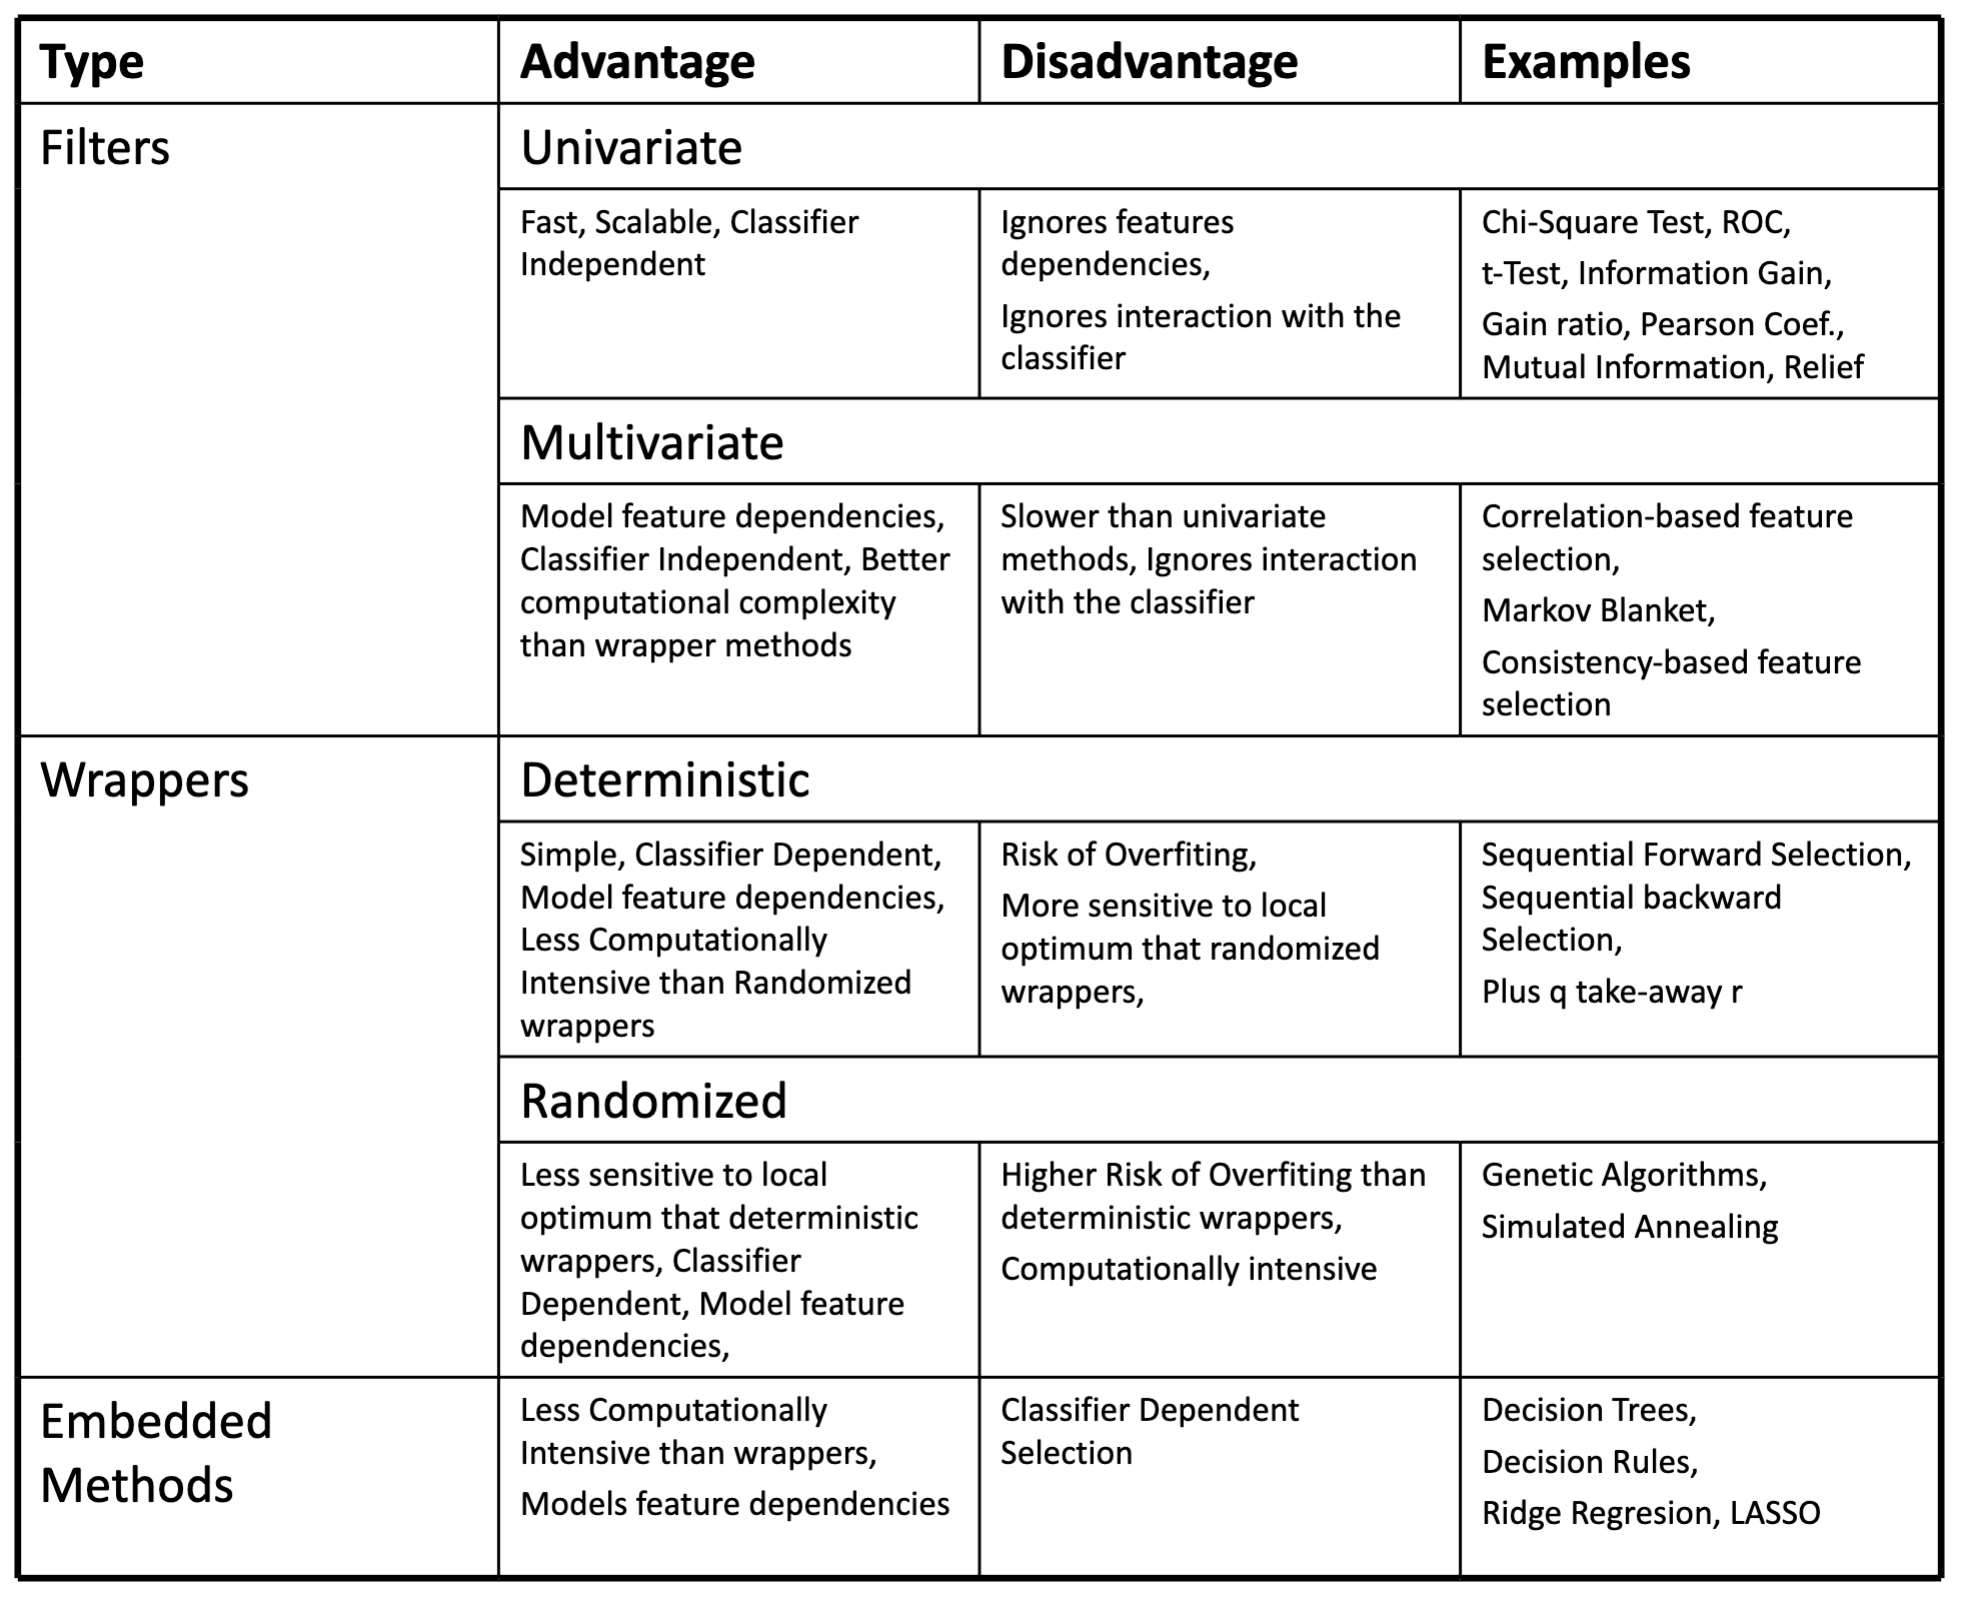
\includegraphics[width=0.8\textwidth]{images/image6.png}
\end{center}

\section*{Filters}
Rank features or feature subsets independently of the learning algorithm (classifier).

\begin{itemize}
    \item \textbf{Advantages:} Fast, Simple, Interpretable, Classifier independence, High dimensionality tolerance
    \item \textbf{Disadvantages:} Ignore interaction with classifiers, ignore feature dependencies.
\end{itemize}

\section*{Univariate Filters}

The relevance of individual feature $X_i$ is determined by how much $X_i$ can explain the output feature $Y$. Statistically this means that we need to assess the (in)dependence of $X_i$ and $Y$. In this context we have two questions:

1. Is $X_i$ independent of $Y$?
2. If $X_i$ and $Y$ are not independent, then how much are they dependent?

We have these scenarios:
\begin{itemize}
    \item The feature $X_i$ is discrete and the feature $Y$ is discrete: Chi-Square Test for Independence, ROC, Information gain and Ratio; Relief; Mutual Information.
    \item The feature $X_i$ is continuous and the feature $Y$ is discrete: t-Test on two means; Relief.
    \item The feature $X_i$ is continuous and the feature $Y$ is continuous: Mutual Information.
\end{itemize}

\section*{Multivariate Filters}
Multivariate Filters rank feature subsets independently on the type of the predictor later used. They operate by searching in the space of possible feature subsets and choosing those of subsets that maximize a given evaluation criterion.

$N$ features, $2^N$ possible feature subsets

\subsection*{Search}
\begin{itemize}
    \item \textbf{Search Direction:} Forward, Backward, Bidirectional
    \item \textbf{Search Strategy:} 
    \begin{itemize}
        \item Deterministic: Hill Climbing, Best First, Exhaustive
        \item Non-deterministic: Genetic
    \end{itemize}
\end{itemize}

\subsection*{Feature Subset Assessment}
Split the data into 3 subsets: training, validation, and test.
\begin{enumerate}
    \item For each feature subset, train predictor on training data.
    \item Select the feature subset which performs best on validation data.
    \item Repeat and average if you want to reduce variance (cross-validation).
    \item Test on test data.
\end{enumerate}

\subsection*{Data Leakage}
Data leakage in validation occurs when information from outside the training fold is used—directly or indirectly—during model training or preprocessing, causing the model to appear more accurate in evaluation than it really is.

\subsection*{Correlation Based Feature Selection}
Evaluation of feature subsets based on the next formula:

$$\text{CFS}(X_i, Y) = \frac{kr_{cf}}{\sqrt{k + (k-1)r_{ff}}}$$

where $S$ is a set with $k$ features, $r_{cf}$ is the average correlation between the features in $S$ and the class feature, and $r_{ff}$ is the average correlation between the features in $S$.

\section*{Wrappers}
Wrappers rank feature subsets w.r.t.\ the predictor used. They operate by searching in the space of possible feature subsets and choosing those of subsets that maximize a given evaluation criterion based on the predictor later used. The evaluation method of the classifier for feature evaluation usually is k-fold cross validation.

\subsection*{Recursive Feature Elimination}
Recursive Feature Elimination is a wrapper that recursively reduces the set of features by eliminating the least important ones based on the ranking provided by a specific model.

\begin{itemize}
    \item \textbf{Feature Dependency:} RFE takes into account the feature dependency assuming that are incorporated in the ranks.
    \item \textbf{Feature Ranking:} Not only does RFE help in selecting important features, but it also ranks all features based on their importance.
    \item \textbf{Handles Multicollinearity:} If some features are correlated, RFE can help in identifying and retaining the most important one among them.
    \item \textbf{Flexibility:} RFE can be used with any model that assigns weights or importance to features, making it versatile.
    \item \textbf{Computationally Intensive:} As RFE involves training the model multiple times (once for each feature), it can be computationally expensive.
    \item \textbf{Model Dependency:} The effectiveness of RFE is tied to the chosen model. A poorly chosen model might lead to sub-optimal feature selection.
    \item \textbf{Stability Issues:} Slight changes in the data can lead to different rankings, especially when features have similar importance.
    \item \textbf{Base Model Selection:} The choice of the model used in RFE is crucial. It's advisable to use a model that naturally provides importance or coefficient values, like decision trees, linear regression, or support vector machines.
\end{itemize}

\section*{Embedded Methods}
White box predictors are actually based on feature selection. So, embedded methods are all the learning algorithms that derive white box predictors. These include: Decision trees and rules, and Shrinkage methods such as ridge regression and LASSO.

\end{lecture}

% Lecture 7
\section{Model Validation}
\label{sec:lecture7}
\begin{lecture}{Lecture 7: Model Validation}
\section*{Model Validation}

\subsection*{Confusion Matrix}

How to validate classifier performance? We use the following confusion matrix (table):

\begin{center}
\begin{tabular}{|c|c|c|}
\hline
\textbf{Actual/Predicted} & \textbf{Pos} & \textbf{Neg} \\ \hline
\textbf{Pos} & TP & FP \\ \hline
\textbf{Neg} & FN & TN \\ \hline
\end{tabular}
\end{center}

Where:
\begin{itemize}
    \item TP: True Positives
    \item FP: False Positives
    \item FN: False Negatives
    \item TN: True Negatives
\end{itemize}

\subsection*{Performance Metrics}

\textbf{Accuracy:} 
$$\text{Accuracy} = \frac{TP + TN}{TP + TN + FP + FN}$$

\textbf{Error Rate:}
$$\text{Error Rate} = 1 - \text{Accuracy} = \frac{FP + FN}{TP + TN + FP + FN}$$

\textbf{Precision:} 
$$\text{Precision} = \frac{TP}{TP + FP}$$

\textbf{Recall (Sensitivity, True Positive Rate):}
$$\text{Recall} = \frac{TP}{TP + FN}$$

\textbf{Specificity (True Negative Rate):}
$$\text{Specificity} = \frac{TN}{TN + FP}$$

\textbf{F1-Score:}
$$F_1 = 2 \times \frac{\text{Precision} \times \text{Recall}}{\text{Precision} + \text{Recall}}$$

\subsection*{ROC Curve}

\begin{itemize}
    \item ROC (Receiver Operating Characteristic) curve plots the True Positive Rate (Sensitivity) against the False Positive Rate (1 - Specificity) at various threshold settings.
    \item The area under the ROC curve (AUC-ROC) provides an aggregate measure of performance across all possible classification thresholds.
    \item A model with perfect discrimination has an AUC of 1.0, while a model with no discrimination has an AUC of 0.5 (a diagonal line).
\end{itemize}

\subsection*{Cross-Validation}

\textbf{K-Fold Cross-Validation:}
\begin{enumerate}
    \item Randomly split the dataset into k equal-sized folds (subsets).
    \item For each fold k:
    \begin{itemize}
        \item Use fold k as the validation set.
        \item Use the remaining k-1 folds as the training set.
        \item Train the model on the training set and evaluate it on the validation set.
    \end{itemize}
    \item Calculate the average performance across all k folds.
\end{enumerate}

\textbf{Stratified K-Fold:} A variation that preserves the percentage of samples for each class in each fold.

\subsection*{Bias-Variance Tradeoff}

\begin{itemize}
    \item \textbf{Bias:} Error due to overly simplistic assumptions in the learning algorithm. High bias can cause underfitting.
    \item \textbf{Variance:} Error due to too much complexity in the learning algorithm. High variance can cause overfitting.
    \item The goal is to find the right balance between bias and variance to minimize total error.
\end{itemize}

\subsection*{Regularization}

Regularization techniques help prevent overfitting by adding a penalty term to the loss function:

\textbf{L1 Regularization (Lasso):}
$$L(\mathbf{w}) = \text{Loss}(\mathbf{w}) + \lambda \sum_{i=1}^n |w_i|$$

\textbf{L2 Regularization (Ridge):}
$$L(\mathbf{w}) = \text{Loss}(\mathbf{w}) + \lambda \sum_{i=1}^n w_i^2$$

\subsection*{Hyperparameter Tuning}

\textbf{Grid Search:} Exhaustive search over a specified parameter grid.

\textbf{Random Search:} Randomly samples parameter combinations from a distribution.

\textbf{Cross-Validation:} Used to evaluate each hyperparameter combination's performance.

\subsection*{Model Comparison}

\begin{itemize}
    \item Compare models using appropriate metrics (e.g., accuracy, F1-score, AUC-ROC).
    \item Use statistical tests (e.g., paired t-test) to determine if differences in performance are statistically significant.
    \item Consider computational efficiency, interpretability, and other practical aspects.
\end{itemize}

\end{lecture}

\end{document}
